 \begin{figure}[t!]
    \centering
    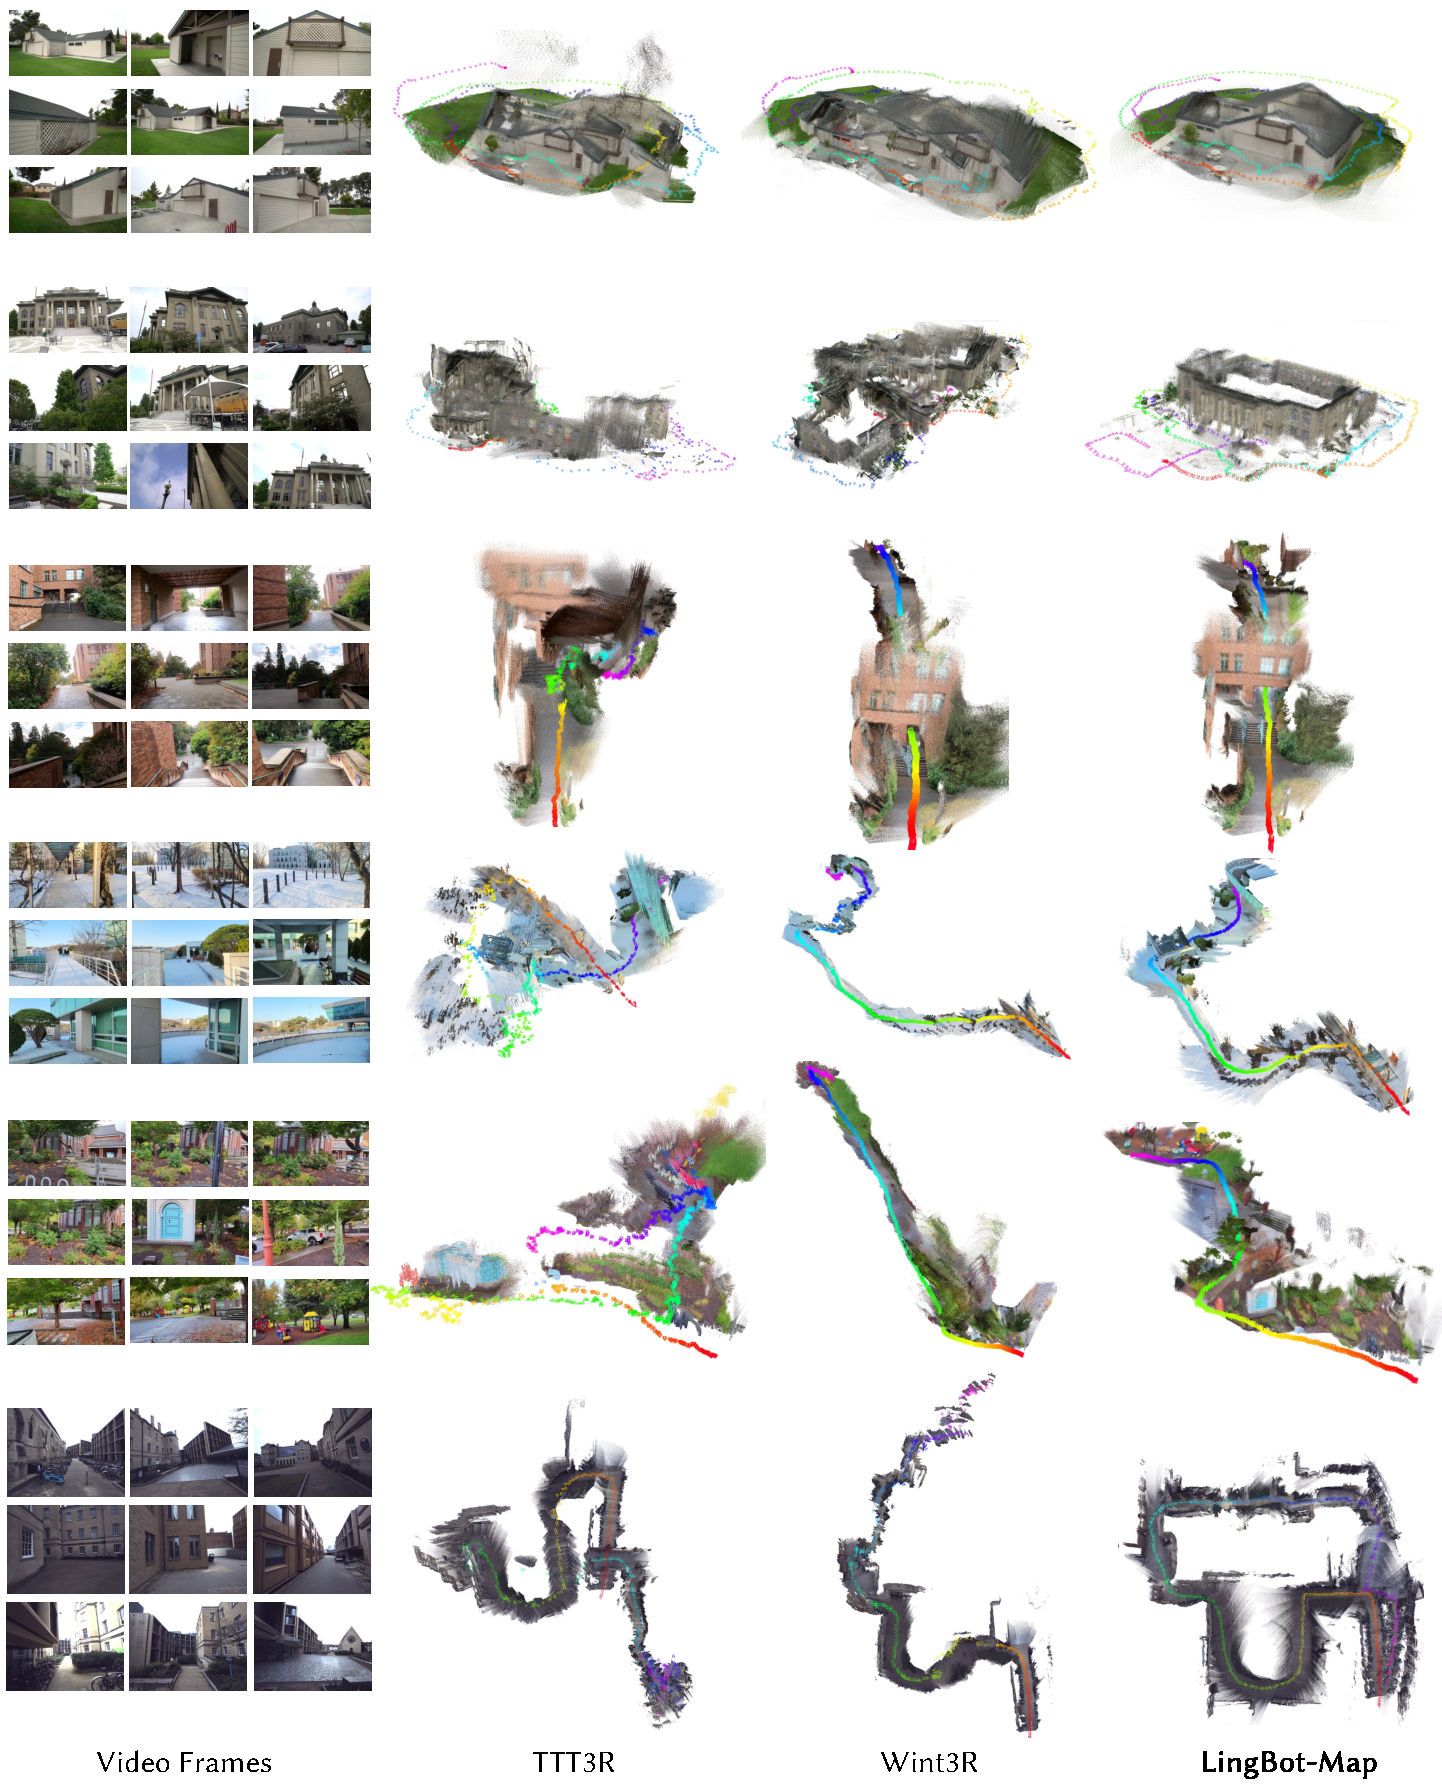
\includegraphics[width=0.98\textwidth]{figures/point_comparison.pdf}

    \caption{\textbf{Qualitative comparison of point cloud reconstruction.}
    LingBot-Map produces geometrically coherent and temporally stable reconstructions, preserving sharp building edges and continuous surfaces even over long sequences with revisits.
    TTT3R and Wint3R suffer from trajectory drift that causes fragmented geometry and duplicated structures, with degradation most severe in complex multi-building scenes (bottom rows).}
    \label{fig:point_comparison}
    \vspace{-1em}
  \end{figure}
